\documentclass[12pt,a4paper]{article}
\usepackage[latin1]{inputenc}
\usepackage{amsmath}
\usepackage{amsfonts}
\usepackage{graphicx}
\usepackage{amssymb}
\usepackage{float}
\usepackage{subfigure}
\usepackage{makeidx}
\author{Giuseppe}
\begin{document}
\section*{Benchmark utilizzato nelle prove}
Il benchmark utilizzato per il testing del sistema di interconnessione del Cell Broadband Engine (CBE) � \textit{danis cycle element}. Esso permette di saturare l'infrastruttura di comunicazione ed � quindi ideale per metterne alla prova le prestazioni.\\
Il benchmark prevede la comunicazione di ciascun Synergistic Processor Element (SPE) con il suo vicino. Ogni SPE esegue il trasferimento, tramite DMA, di blocchi di dati di dimensione di 64 byte (o 128, o 256, ecc\ldots) verso la Local Store (LS) della SPE sua vicina. Questa configurazione � quella che modella il caso pi� favorevole, in cui le immagini dell'applicazione vengono distribuite in modo tale che le SPE che cooperano per il processing dei dati siano adiacenti sul ring. Sar� in seguito presentata anche la configurazione che modella il caso peggiore, ovvero quello nel quale ogni SPE deve comunicare con la SPE che si trova alla massima distanza. 

\section*{Topologie di rete oggetto delle analisi}

Vengono di seguito descritte le diverse configurazioni topologiche dell'Element Interconnect Bus (EIB) e in aggiunta anche una soluzione a pacchetti basata sull'architettura \textit{$\times$pipes NoC}.\\
Per quanto riguarda EIB, l'analisi si basa sull'osservazione delle prestazioni, sia in termini di latenza media e massima per ogni trasferimento, che in termini di tempo (in numero di cicli di sistema) di esecuzione dell'applicazione al variare del numero di ring e del numero massimo di transazioni che possono coesistere su ciascun ring. Le configurazioni analizzate sono:
\begin{itemize}
 	\item EIB\_2\_RING\_2\_MAX\_TRANS: 2 ring, 2 max coexisting transactions;
	\item EIB\_2\_RING\_2\_MAX\_TRANS: 2 ring, 5 max coexisting transactions;
	\item EIB\_2\_RING\_2\_MAX\_TRANS: 4 ring, 2 max coexisting transactions;
	\item EIB\_4\_RING\_5\_MAX\_TRANS: 4 ring, 5 max coexisting transactions;
	\item EIB\_8\_RING\_2\_MAX\_TRANS: 8 ring, 2 max coexisting transactions;
	\item EIB\_8\_RING\_5\_MAX\_TRANS: 8 ring, 5 max coexisting transactions.
\end{itemize}
Per la soluzione a pacchetti $\times$pipes:
\begin{itemize}
 	\item Spidergon
 	\item Mesh $5 \times 2$ 
	\item Torus
	\item Crossbar
\end{itemize}
Per tutte queste ultime sono stati usati i seguenti parametri progettuali:
\begin{itemize}
	\item trasferimento BURST;
	\item MDATAWD pari a 128 bit;
	\item FLITWIDTH tale da consentire il trasferimento di 128 bit a ogni BURST; 
	\item controllo di flusso STALL\&GO.
\end{itemize}

\section*{Risultati simulazioni: best case}

Il miglioramento delle prestazioni di EIB pu� essere ottenuto attraverso l'aumento del numero di ring e del numero massimo di transazioni che possono coesistere su ciascun ring. A noi interessa valutare tale miglioramento e confrontarlo con quello ottenibile da una soluzione alternativa a pacchetti.\\
In figura~\ref{fig:improv-1hop} viene riportato il miglioramento percentuale delle prestazioni, in termini di cicli di esecuzione dell'applicazione, rispetto alla topologia di riferimento EIB\_4\_RING\_5\_MAX\_TRANS, che � anche quella utilizzata nella versione commerciale con la quale � equippaggiata la PlayStation3.
\begin{figure}[H]
	\begin{center}
	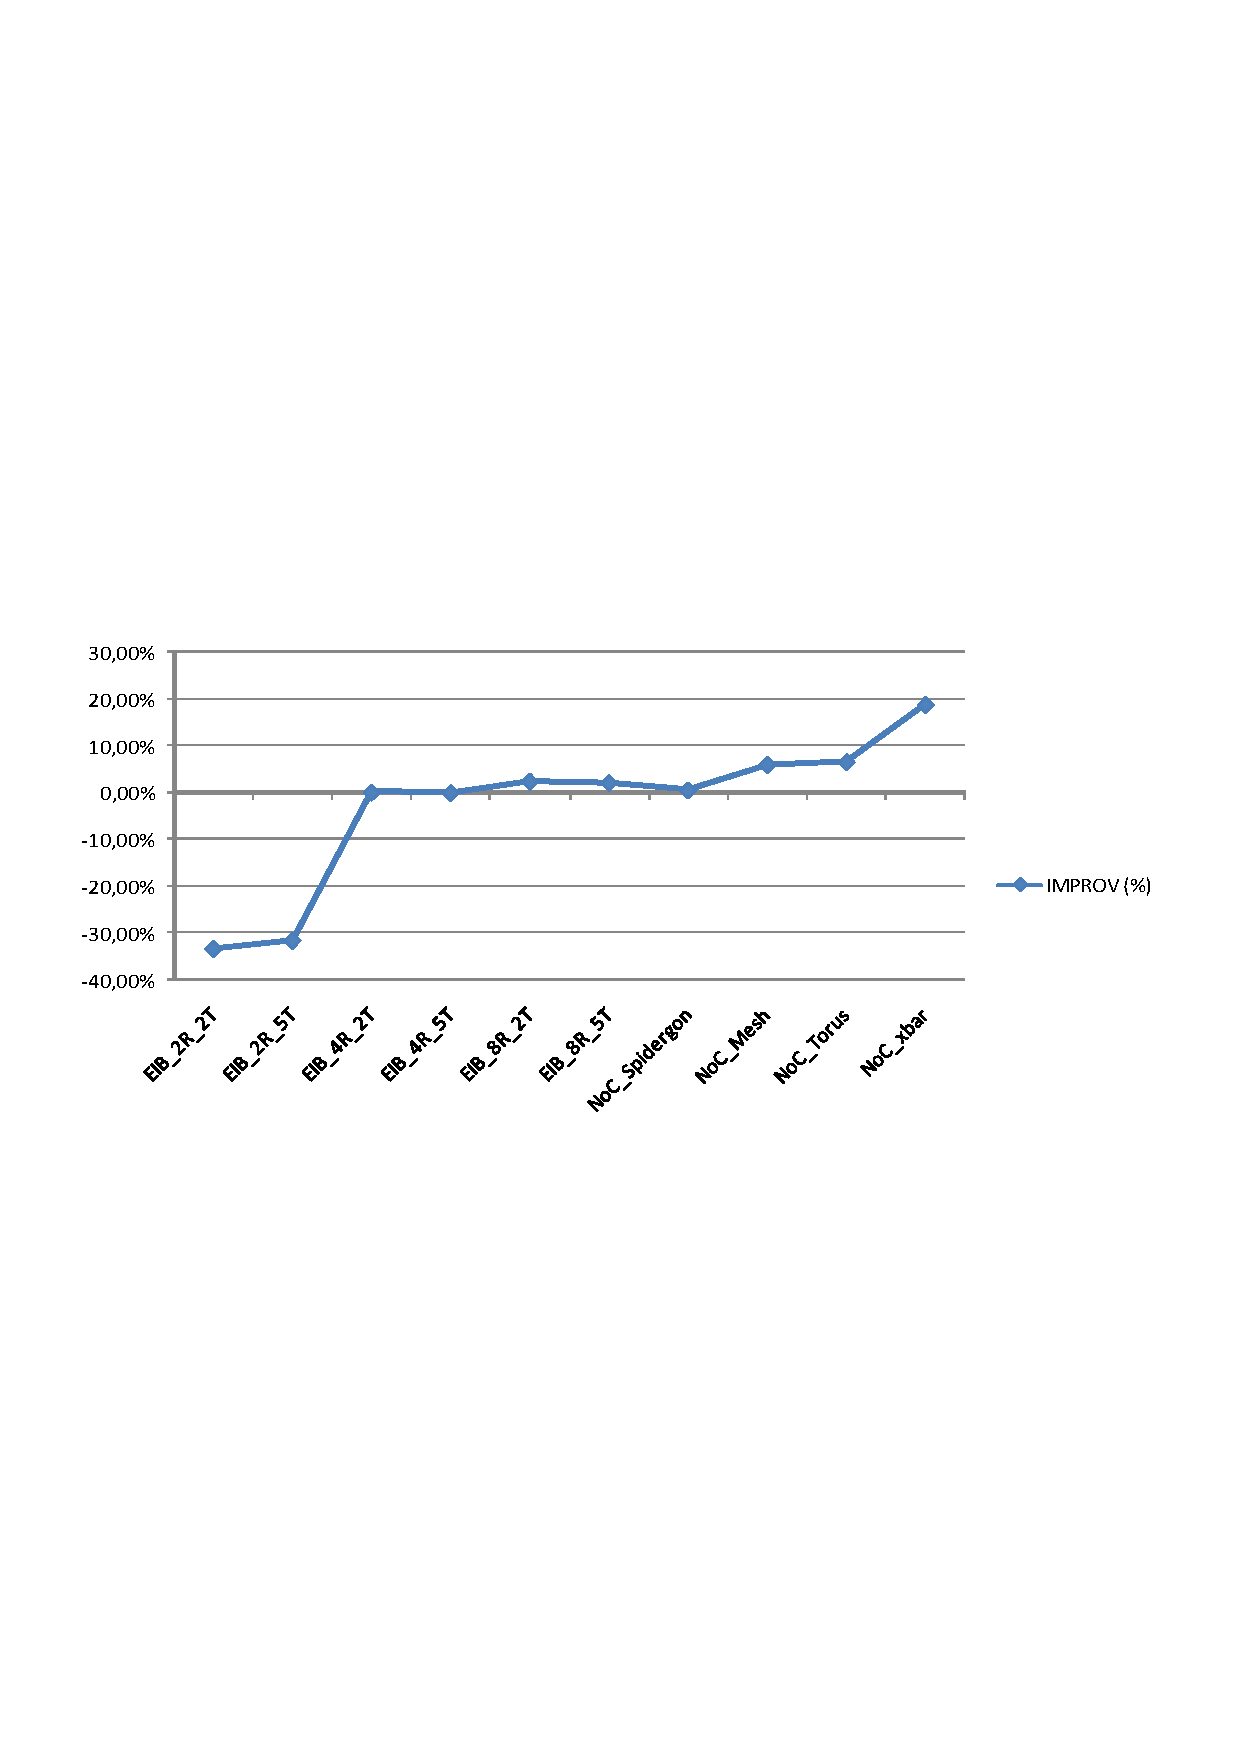
\includegraphics[width=13.5cm]{figure/improvement-1hop}
	\end{center}
	\caption{Miglioramento percentuale delle prestazioni, nel best case, al variare della topologia}
	\label{fig:improv-1hop}
\end{figure}
In figura, per quanto riguarda EIB, si pu� osservare la rapida riduzione del tempo di esecuzione passando dalla configurazione a 2 ring e 2 transazioni a quella con 4 ring, un miglioramento di oltre il 20\%. Questo miglioramento continua, anche se in modo meno incisivo, se si va verso topologie con 8 ring (miglioramenti che non superano il 2.5\%). Si pu� ridurre ulteriomente il tempo di esecuzione abbandonando la soluzione basata su ring per passare a quella basata su pacchetti. Con le topologie Spidergon, Mesh, Torus e Crossbar si ottengono miglioramenti, rispettivamente, di circa l'11\% per le prime tre e 16\% per l'ultima. \\
Questi risultati avvallano la scelta di 4 ring per la versione commerciale del Cell poich� le soluzioni con 8 ring non danno miglioramenti consistenti a fronte di un aumento della potenza dissipata e dell'area sul chip.
L'utilizzo di una soluzione alternativa a pacchetti � invece auspicabile alla luce dei risultati ottenuti. 
\section*{Risultati simulazioni: worst case}
Vediamo ora di valutare le prestazioni nel caso in cui la distribuzione delle immagini tra le varie SPE non sia ottimale. Mentre nel best case le SPE potevamo comunicare tra loro contemporaneamente senza sovrapporsi, nel worst case i percorsi che le SPE utilizzano per comunicare si possono sovrapporre e causare \emph{overlapping}. In questo caso, si aspetta che la coppia che detiene la risorsa la rilasci. Da ci� si deduce che l'unica via per ridurre il tempo di esecuzione, nel caso di EIB, � quella di aumentare il numero di ring. In figura~\ref{fig:improv-5hop} � riportato l'andamento delle prestazioni nel worst case.
\begin{figure}[H]
	\begin{center}
	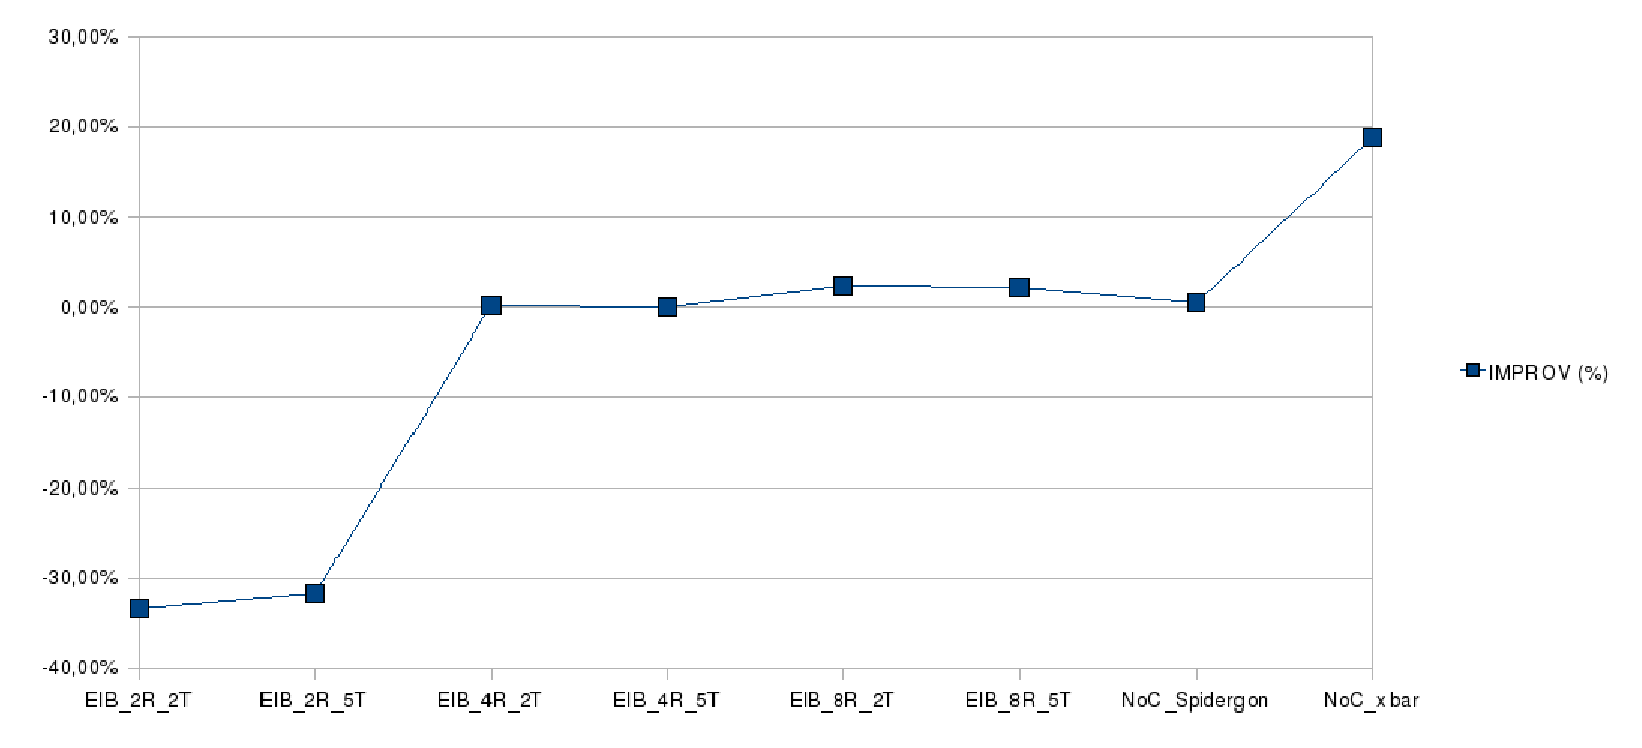
\includegraphics[width=13.5cm]{figure/improvement-5hop}
	\end{center}
	\caption{Miglioramento percentuale delle prestazioni, nel worst case, al variare della topologia}
	\label{fig:improv-5hop}
\end{figure}
Come si pu� osservare, ancora una volta, si ha un forte miglioramento se si passa da 2 ring a 4 ring (miglioramento di oltre il 30\%), mentre aumentando ulteriormente il numero di ring a 8 non si ottiene vantaggio significativo. A differenza del best case, la Spidergon riporta prestazioni paragonabili a quelle di EIB, la Mesh e la Torus mantengono un lieve vantaggio rispetto a quest'ultimo, mentre la Crossbar ancora una volta fornisce le prestazioni migliori, poich� la latenza in quest'ultima � indipendente dalla disposizione delle immagini. 

\section*{Confronto delle prestazioni tra best case e worst case}
E' interessante anche valutare il peggioramento delle prestazioni tra best case e worst case per le varie topologie. La figura~\ref{fig:improv-1hop-5hop} riporta il peggioramento percentuale prendendo come riferimento il caso migliore per ciascuna topologia.
\begin{figure}[H]
	\begin{center}
	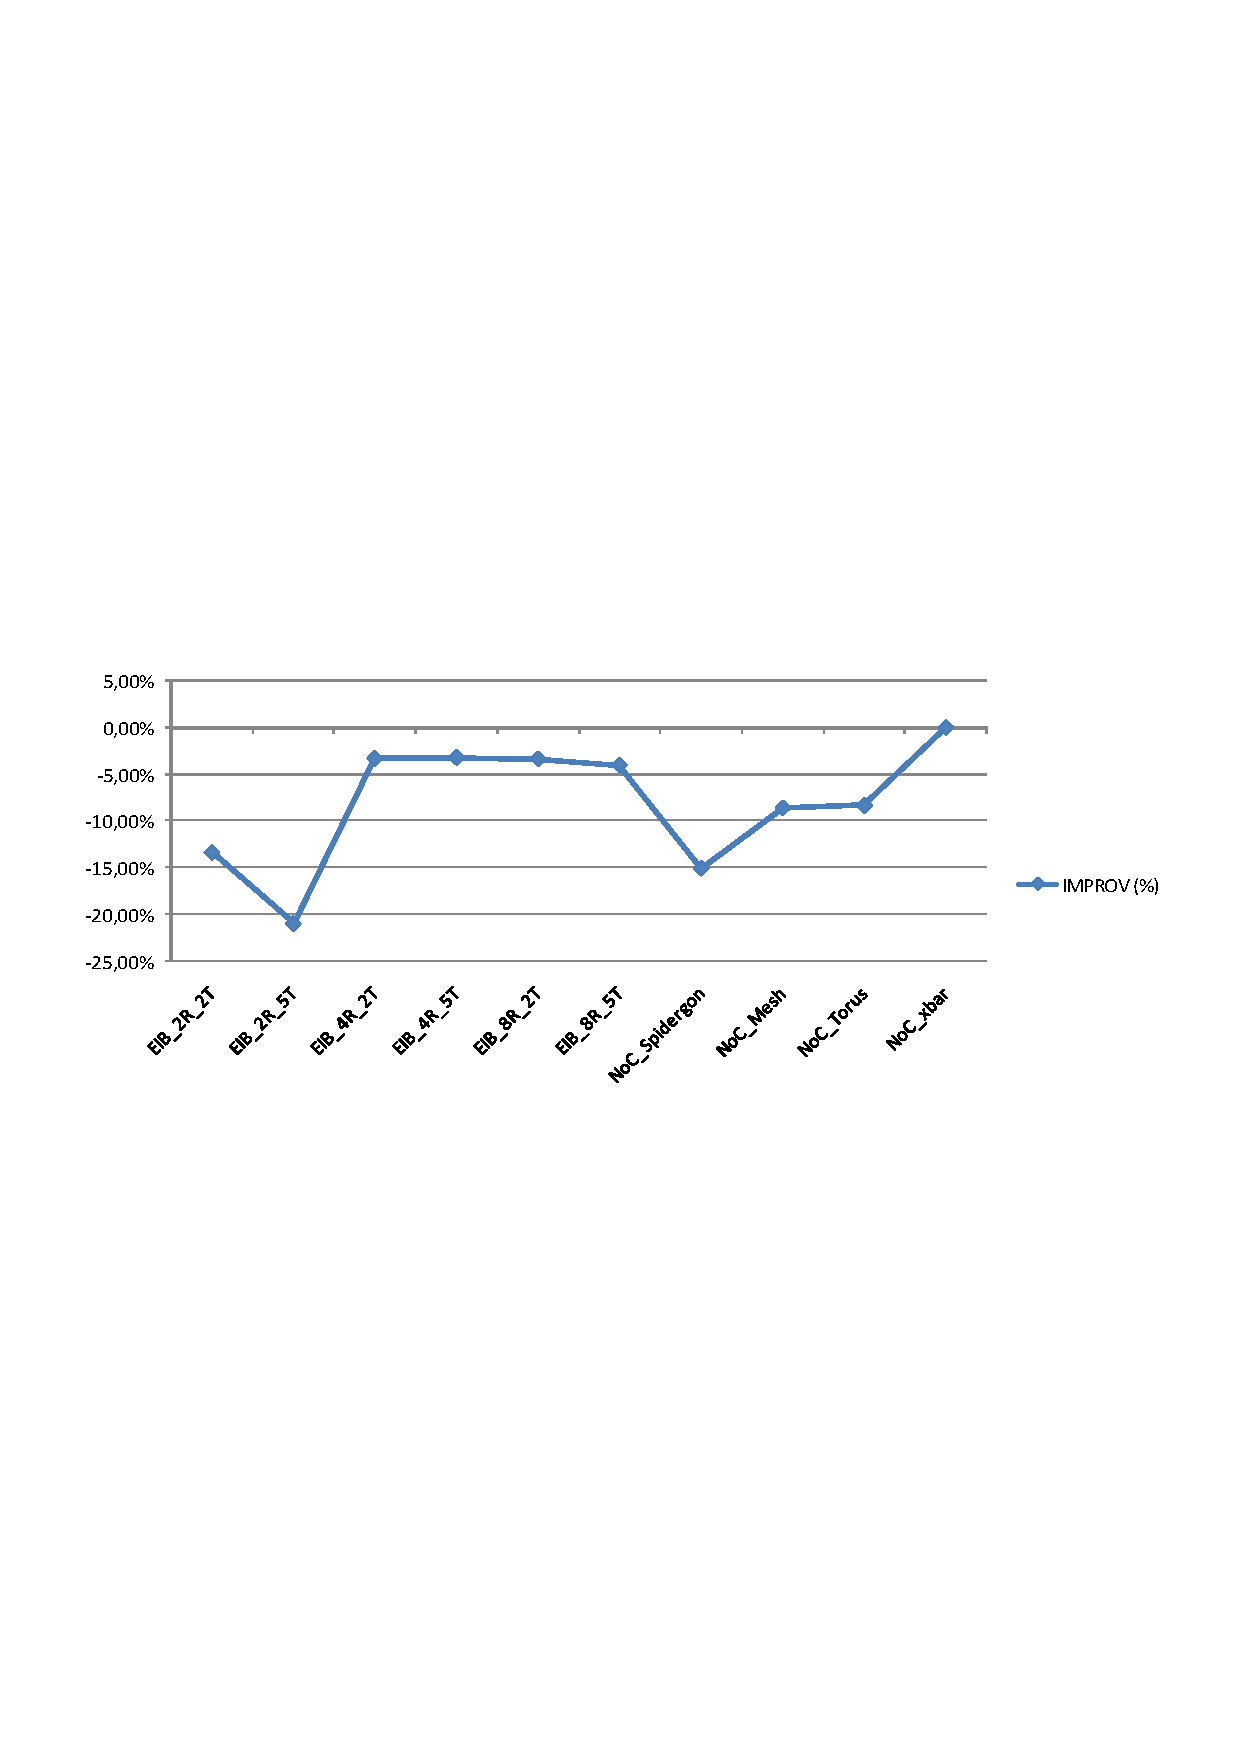
\includegraphics[width=13.5cm]{figure/improvement-1hop-5hop}
	\end{center}
	\caption{Peggioramento percentuale per worst case rispetto al best case}
	\label{fig:improv-1hop-5hop}
\end{figure}
Come prevedibile, abbiamo un peggioramento molto forte per le soluzioni EIB a 2 ring, mentre per quelle con 4 e 8 ring il deterioramento � meno marcato. Per quanto riguarda la NoC, la Spidergon perde rispetto al best case di circa il 15\%, mentre la Crossbar resta stabile poich� le latenze non dipendono dalla distribuzione delle immagini. Tra queste ultime due si posizionano la Mesh e la Torus che perdono l'8\% ciascuna. \\ 
Da ci� si evince come l'utilizzo di una topologia Spidergon porti vantaggi maggiori quando la distribuzione delle immagini � ottimizzata tra le SPE; nonostante il forte peggioramento osservabile nel worst case, tale topologia continua comunque a offrire prestazioni paragonabili a quelle di EIB con 4 e 8 ring. Meglio di questa fanno la Mesh e la Torus che forniscono prestazioni pi� elevate nel worst case. La Crossbar rappresenta, evidentemente, il caso ideale di interconnessione, ma � difficilmente utilizzabile nella pratica. 
\end{document}